\documentclass[a4paper, 10pt]{article}

\usepackage{global-macros}
\usepackage{fullpage}
\usepackage{sectsty}

\allsectionsfont{\large\sffamily}

\title{{\Large\bfseries\sffamily Bayesian Statistics --- Assignment 2} \\ \large\sffamily On the Bayesian Lasso}
\author{\normalsize Caio Peixoto}
\date{\normalsize\today}

\begin{document}

\maketitle

\tableofcontents

\section{LASSO regression and the Laplace prior}
In\footnote{Corresponds to items a) and b).} this work we will study the usual linear regression model, given by 
\begin{equation}
    \by \mid \mu, \betabold, \bX, \sigma^2 \sim \Normal(\mu \ones_{ n } +  \bX \betabold, \sigma^2 \eye_n)
    \label{eq: likelihood}
,\end{equation}
where $ \bX \in \R^{n \times p}, \betabold \in \R^{ p }, \mu \in \R $, $ \ones_{ n } $ denotes the vector in $ \R^{ n } $ with all coordinates set to $ 1 $ and $ \eye_{ n } $ denotes the $ n $-dimensional identity matrix.
The goal is to conduct inference on $ \mu, \betabold $ and $ \sigma^2 $, and we will follow the Bayesian approach in \cite{parkcasella2008bayesianlasso}.

In \cite{tibshirani1994lasso}, the author presented an estimator for $ \betabold $ and $ \mu $, called the LASSO\footnote{\emph{Least absolute shrinkage selection operator.}}, with the following definition:
\begin{equation}
    ( \hat{ \betabold }_{ \lasso }, \hat{ \mu }_{ \lasso } )
    = \argmin_{ \norm{ \betabold }_{ 1 } \leq t, \mu \in \R } \ \norm{\by - \mu \ones_{ n } - \bX \betabold}_2^2
    \label{eq: lasso constrained}
,\end{equation}
where $ t > 0 $ is a tuning parameter.
His goal was to address two of the main problems of the usual OLS estimator, which does not include the $ L^{ 1 } $ norm constraint: \emph{high variance}, which lowers prediction accuracy, and \emph{lack of interpretability}, particularly when the number of predictors is high.
The effect produced by the $ L^1 $ constraint is the shrinkage of the overall coefficient magnitude and, more importantly, the collapse of the less important coefficients to exactly $ 0 $.
This effect introduces bias in the estimation, but the gain in variance is enough to improve predictive performance.
Furthermore, it provides a principled way to perform variable selection, by discarding the variables whose coefficients were collapsed to $ 0 $.

One might wonder what is special about the $ L^1 $ norm, since this collapsing behavior is not observed for the Ridge estimator, which uses $ L^2 $ constraint instead of $ L^1 $.
It turns out the reason is geometric.
The $ L^1 $ ball in $ \R^{ p } $ has sharp edges and vertices, in contrast with the smooth surface of the $ L^2 $ ball.
When solving problem (\ref{eq: lasso constrained}), the solution will often be located on an edge of the $ L^1 $ ball of radius $ t $.
Along these edges, one or more coefficients are exactly zero, which produces the collapsing effect.

Although the methodology in \cite{tibshirani1994lasso} is classical, in Section 5 the authors point out that problem (\ref{eq: lasso constrained}) is equivalent to MAP estimation when employing a Laplace prior.
To see this, note that the constrained optimization problem is equivalent to the following regularized version:
\begin{equation*}
    \argmin_{ \betabold \in \R^{ p }, \mu \in \R } \norm{ \by - \mu \ones_{ n } - \bX \betabold }_{ 2 }^{ 2 } + \lambda \norm{ \betabold }_{ 1 }
,\end{equation*}
where $ \lambda $ depends on $ t $.
Much like the squared Euclidean norm in the objective corresponds to the normal likelihood, the $ L^1 $ norm can be seen as the log of the kernel of the Laplace distribution.
Hence, the LASSO is the MAP estimator when the prior for $ \betabold $ is chosen as
\begin{equation*}
    \pi ( \betabold ) = \left( \frac{ \lambda }{ 2 } \right)^n \exp \left\{ - \lambda \norm{ \betabold }_{ 1 } \right\}
.\end{equation*}
Expanding upon this observation, in \cite{parkcasella2008bayesianlasso} the authors discuss a Bayesian formulation for LASSO regression by employing the following joint prior on $ \betabold $ and $ \sigma $:
\begin{align}
    \begin{split}
        \pi ( \sigma^2 ) &\propto \frac{ 1 }{ \sigma^2 } \cdot \ind \{ \sigma^2 > 0 \}, \\
        \pi ( \betabold \mid \sigma^2 ) &= \left( \frac{ \lambda }{ 2 \sqrt{ \sigma^2 } } \right)^{ n } \exp \left\{ - \frac{ \lambda }{ \sqrt{ \sigma^2 } } \norm{ \betabold }_{ 1 } \right\},
    \end{split}
    \label{eq: conditional laplace prior}
\end{align}
where $ \lambda $ is a hyperparameter which can be given a hyperprior or be estimated using marginal maximum likelihood methods.
The choice for a Laplace prior for $ \betabold $ is necessary to recover the LASSO estimator as the MAP.
With a normal prior, for instance, the MAP would become the Ridge regression estimator.
This conditional structure in the prior is justified in \cite{parkcasella2008bayesianlasso} by a computational argument: without it, the posterior may exhibit multimodality, which can pose difficulties for MCMC sampling schemes such as the Gibbs sampler.
From a statistical perspective, this prior encapsulates the idea that the larger $ \sigma^2 $ is, the less informative the prior on $ \betabold $ should be.
This makes \emph{some} sense, since, for more spread out $ y $ values, we would like the prior not to be as restrictive and not to ``get in the way'' of the likelihood.
On another note, it would also be reasonable not to assume $ \betabold $ and $ \sigma^2 $ depend on each other in any way a \emph{priori}.
Anyway, since we are following the methodology of \cite{parkcasella2008bayesianlasso}, our prior of choice will be (\ref{eq: conditional laplace prior}).

The main motivation for this Bayesian formulation is the already mentioned fact that the LASSO estimator is recovered as the MAP.
However, Bayesian estimation goes far beyond maximizing the posterior, and one might wonder if other forms of inference based on the prior (\ref{eq: conditional laplace prior}) exhibit shrinkage-like properties.
This, among other things, is what we will investigate in the following sections.
Apart from the usual advantages of having a full probability distribution describing our belief about the parameters, it is not clear if this Bayesian approach does what we might desire it to do, e.g., produce credibility intervals which include $ 0 $ for the irrelevant covariates and exclude it for the relevant ones.
In fact, there are statisticians which assert that the Bayesian LASSO simply \emph{does not work}, as can be seen, for instance, in \cite{simpson2021}.
Simpson's argument is that the prior (\ref{eq: conditional laplace prior}) either shrinks \emph{almost all} parameters to $ 0 $, or does not produce \emph{any shrinkage at all}.

% \begin{itemize}
%     \item Introduce notation for linear regression;
%     \item Explain the Lasso regularization;
%     \item Explain why the L1 norm produces shrinkage;
%     \item Show how the LASSO estimator is the MAP estimator when using the Laplace prior;
%     \item Explain the conditional structure of the Laplace prior;
%     \item Comment on possible advantages of having a full probability distribution for the parameters;
%     \item Talk about possible disadvantages of using the Laplace prior, allude to excessive shrinkage in the experiments;
% \end{itemize}

\section{The Gibbs sampler}
In\footnote{Corresponds to items c) and d).} \cite{parkcasella2008bayesianlasso}, the authors propose a Gibbs sampler to draw samples from the posterior.
This sampler uses the following decomposition of the Laplace distribution: if $s \sim \Exp(a^2 / 2)$\footnote{This is the \emph{rate} parameter} and $ z \mid s \sim \Normal(0, s) $, then, marginally, $ z \sim \Laplace(a) $, that is,
\begin{equation*}
    p ( z ) = \frac{ a }{ 2 } \exp \{ - a \abs{ z } \}
.\end{equation*}
Using this decomposition, one may rewrite the model given by (\ref{eq: likelihood}) and (\ref{eq: conditional laplace prior}) with auxiliary variables $ \tau_{ 1 }^2, \dots, \tau_{ p }^2 $:
\begin{align*}
    \by \mid \mu, \betabold, \bX, \sigma^2 &\sim \Normal(\mu \ones_{ n } +  \bX \betabold, \sigma^2 \eye_n), \\
    \betabold \mid \sigma^2, \tau_{ 1 }^2, \dots, \tau_{ p }^2 &\sim \Normal (\zeros_{ p }, \sigma^2 \bD_{ \tau }), \\
    \bD_{ \tau } &= \diag (\tau_{ 1 }^2, \dots, \tau_{ p }^2), \\
    \tau_{ i }^2 &\iid \Exp(\lambda^2 / 2),
\end{align*}
and $ \sigma^2 $ is distributed independently of $ \tau_{ 1:p }^2 $ according to a distribution $ \pi $ with positive support, while $ \mu $ is given an independent, flat, prior.
Park and Casella chose to use $ \pi \propto \frac{ 1 }{ \sigma^2 } \ind \{ \sigma^2 > 0 \} $, but, as they mentioned in \cite{parkcasella2008bayesianlasso}, any inverse-gamma prior could be used without affecting conjugacy.
This is a way to introduce subjective knowledge about $ \sigma^2 $ to the prior.
It is necessary to introduce the auxiliary variables $ \tau_{ 1 }^2, \dots, \tau_{ p }^2 $ because the $ L^1 $ norm which appears inside the exponential in the Laplace distribution makes the full conditional of $ \betabold $ hard to sample from.
With this new hierarchical structure, the full conditional of $ \betabold $ is multivariate normal, while that of $ \sigma^2 $ and $ 1/\tau_{ i }^2 $ are inverse gamma and inverse Gaussian, respectively.
Of course, this is only needed if one is interested in fully exploring the posterior distribution.
If all one desires is to compute the MAP, then it is best to go back to the prior in (\ref{eq: conditional laplace prior}) and use any available package to obtain the LASSO estimator.

The intercept parameter, $ \mu $, is only related to the location of $ \by $, and, thus, does not contain any information on which covariates are relevant and which are not.
If the goal of the data analyst is only to analyze the effect of each covariate on the outcome, there is no reason to conduct inference on (and, hence, sample from) the intercept $ \mu $.
It can be easily marginalized from the joint distribution of data and parameters, and this was the rout taken in \cite{parkcasella2008bayesianlasso}.
The authors mention that, should one desire to sample from $ \mu $, its full conditional is normal with mean $ \bar{ \by } $ and variance $ \sigma^2/n $.


% \begin{itemize}
%     \item Explain the sampling hierarchy suggested by Park and Casella.
%     \item Modify the hierarchy to facilitate MAP estimation;
%     \item Discuss how one should include information about the measurement noise parameter?
%     \item Discuss why marginalize $\mu$ in the computation and when that is and is not desirable;
%     \item Show how to recover inferences about $ \mu  $ in the marginalized case.
% \end{itemize}

\section{But can it actually shrink?}
\label{sec: artificial data experiments}
In\footnote{Corresponds to item e).}\footnote{All code for the experiments in Sections \ref{sec: artificial data experiments} and \ref{sec: diabetes data experiment} is openly available in \href{https://github.com/Caioflp/bayesian-statistics-final-assignment}{Github} } this section, we will investigate the shrinking properties of the Bayesian LASSO using the artificial data scenarios in presented in the Section 7.2 of \cite{tibshirani1994lasso}.
All the scenarios consist of generating $ n $ samples from the model in (\ref{eq: likelihood}), where the lines of $ \bX $ are independent samples from a multivariate normal distribution.
We considered two sample sizes: $ n = 20 $ and $ n = 100 $.
For the prior distribution, we employed the prior in (\ref{eq: conditional laplace prior}), with an additional $ \distgamma (\delta, r) $ prior\footnote{Here, $ \delta $ and $ r $ are the \emph{shape and rate} parameters, respectively. This is the \emph{opposite} of what is done in \cite{parkcasella2008bayesianlasso}, however, I realized this mistake far too late to fix it. Fortunately, the only place where this might be annoying is in the next section.} on $ \lambda^2 $ (not $\lambda$), as suggested in Section 3.2 of \cite{parkcasella2008bayesianlasso}.
We specified a weakly-informative prior by choosing $ \delta = 1.0 $ and $ r = 0.1 $.
The sampling scheme we chose was NUTS-HMC, utilized through \texttt{Stan} \cite{stan2024} and \texttt{CmdStanPy}.
For each dataset, we sampled from $ 5 $ chains, using $ 1000 $ warm-up samples and $ 10 000 $ samples from (hopefully) the posterior.
On a last note, we also standardized the columns of $ \bX $ to have mean $ 0 $ and variance $ 1 $.
This is a good practice also employed in \cite{parkcasella2008bayesianlasso}, as it puts all covariates in the same scale.
If one of the betas was much smaller than the other ones simply because of the larger scale of the corresponding covariate, then it might be incorrectly shrunk to $ 0 $ by the LASSO regression.

\subsection*{Scenario 1}

For this scenario, the parameters were
\begin{align*}
    \betabold &= (3, 1.5, 0, 0, 2, 0, 0, 0) \\
    \sigma &= 3
.\end{align*}
The correlation between $ x_{ i } $ and $ x_{ j } $ was set to $ \rho^{ \abs{ i - j } } $, with $ \rho = 0.5 $.
All $ (x_{ i })_{ 1 \leq i \leq 8 } $ had mean $ 0 $.

Effective sample size and $ \hat{ R } $ statistics are in Table \ref{tab: Eff and Rhat scenario 1}.
We can see that, for both values of $ n $, the $ \hat{ R } $ values are very close to one, indicating that we are indeed sampling from the posterior.
The effective sample sizes are also quite high, which allows us to trust the credibility intervals computed from these samples.
\begin{table}[htb]
    \centering
    \begin{tabular}{lrr}
& $ n = 20 $ & \\
\toprule
 & N\_Eff & R\_hat \\
\midrule
lp\_\_ & 15200.000000 & 1.000000 \\
mu & 47660.000000 & 1.000000 \\
beta[1] & 31305.000000 & 1.000000 \\
beta[2] & 30485.000000 & 1.000000 \\
beta[3] & 33833.000000 & 1.000000 \\
beta[4] & 39068.000000 & 1.000000 \\
beta[5] & 36640.000000 & 0.999900 \\
beta[6] & 35091.000000 & 1.000000 \\
beta[7] & 33731.000000 & 1.000000 \\
beta[8] & 35182.000000 & 1.000000 \\
sigma & 32499.237400 & 1.000100 \\
lambda & 36077.141000 & 1.000000 \\
\bottomrule
\end{tabular}

    \quad
    \begin{tabular}{lrr}
& $ n = 100 $ &
\toprule
 & N\_Eff & R\_hat \\
\midrule
lp\_\_ & 19470.000000 & 1.000000 \\
mu & 54950.000000 & 1.000000 \\
beta[1] & 41583.000000 & 1.000000 \\
beta[2] & 38976.000000 & 1.000000 \\
beta[3] & 32296.000000 & 1.000000 \\
beta[4] & 35541.000000 & 0.999900 \\
beta[5] & 36941.000000 & 1.000000 \\
beta[6] & 34982.000000 & 1.000000 \\
beta[7] & 31183.000000 & 1.000000 \\
beta[8] & 33972.000000 & 1.000000 \\
sigma & 45289.799000 & 1.000000 \\
lambda & 44630.841000 & 1.000000 \\
\bottomrule
\end{tabular}

    \caption{Effective sample sizes and $ \hat{ R } $ statistics for Scenario 1, reported with four significant digits.}
    \label{tab: Eff and Rhat scenario 1}
\end{table}
In order to further assess chain mixing, we show trace plots of the parameters in Figure \ref{fig: traceplots scenario 1}.
From them, we can see that the chains are generally well mixed for both dataset sizes.
\begin{figure}[htb]
    \begin{center}
        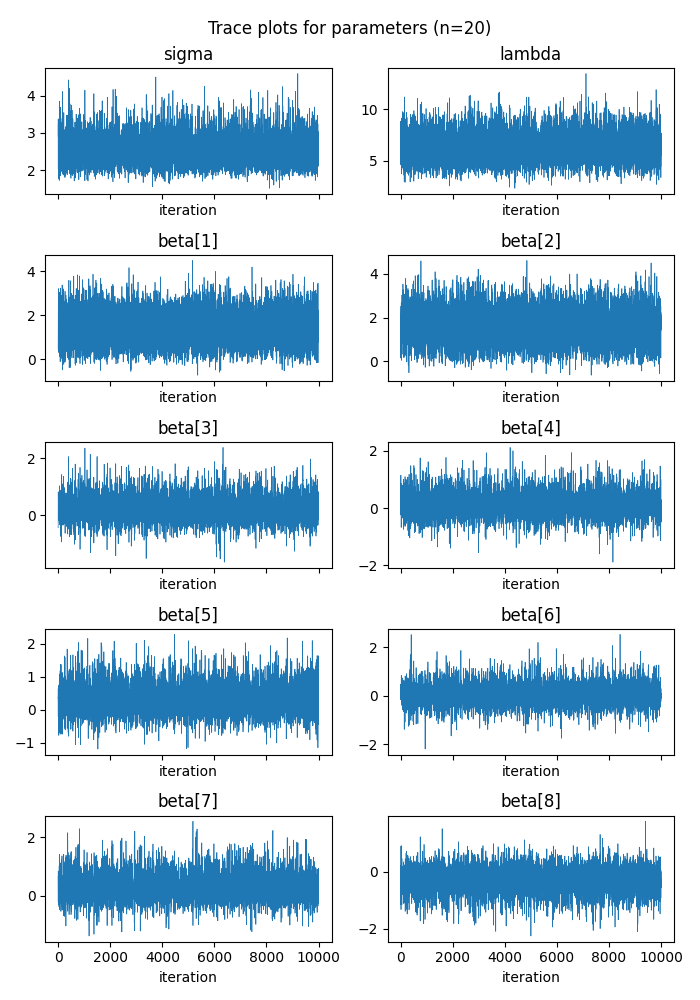
\includegraphics[height=.4\textheight]{../outputs/artificial_scenarios_n=20/scenario_1/traceplots.png}
        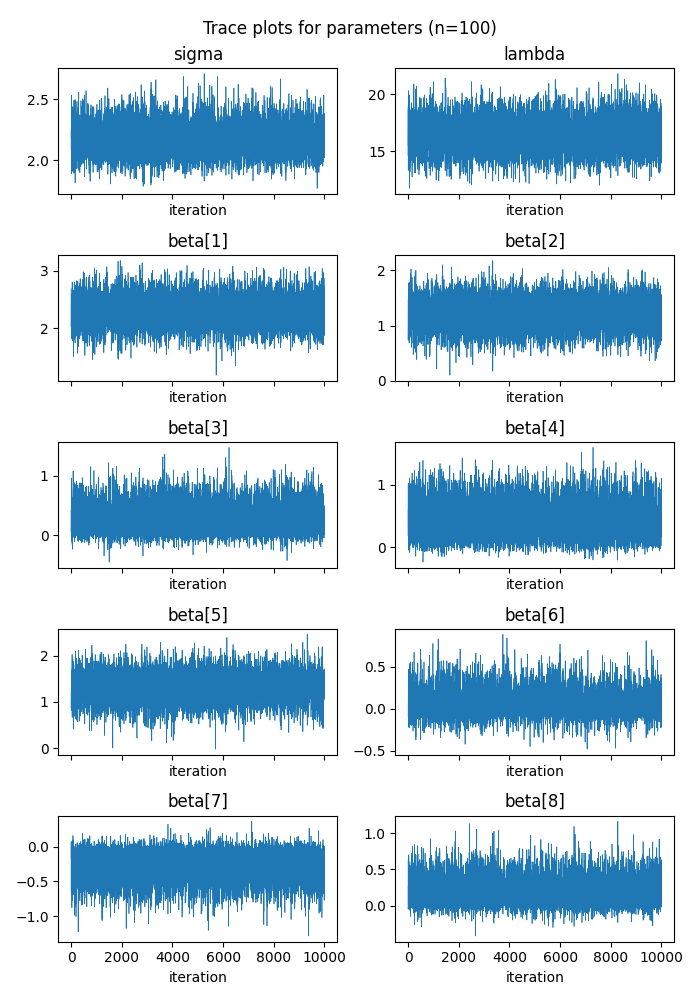
\includegraphics[height=.4\textheight]{../outputs/artificial_scenarios_n=100/scenario_1/traceplots.png}
    \end{center}
    \caption[Trace plots for the parameters in Scenario 1.]{Trace plots for the parameters in Scenario 1. Each plot is from one of the 5 chains, chosen randomly and uniformly.}
    \label{fig: traceplots scenario 1}
\end{figure}
As a final diagnostic, we also conducted a posterior predictive check, whose results are in Figure \ref{fig: posterior predictive check scenario 1}.
To do this, for each sample from the posterior, we sampled $ \by $ according to (\ref{eq: likelihood}) and plotted a histogram of the coordinates.
The actual data is included for comparison.
We can see that there is little resemblance between actual and simulated data for $ n = 20 $, but the situation is better for $ n = 100 $.
This can be due to the large variance ($ \sigma^2 = 9 $) in the data generating process, which makes it hard to extract information from datasets with few samples.
\begin{figure}[htb]
    \begin{center}
        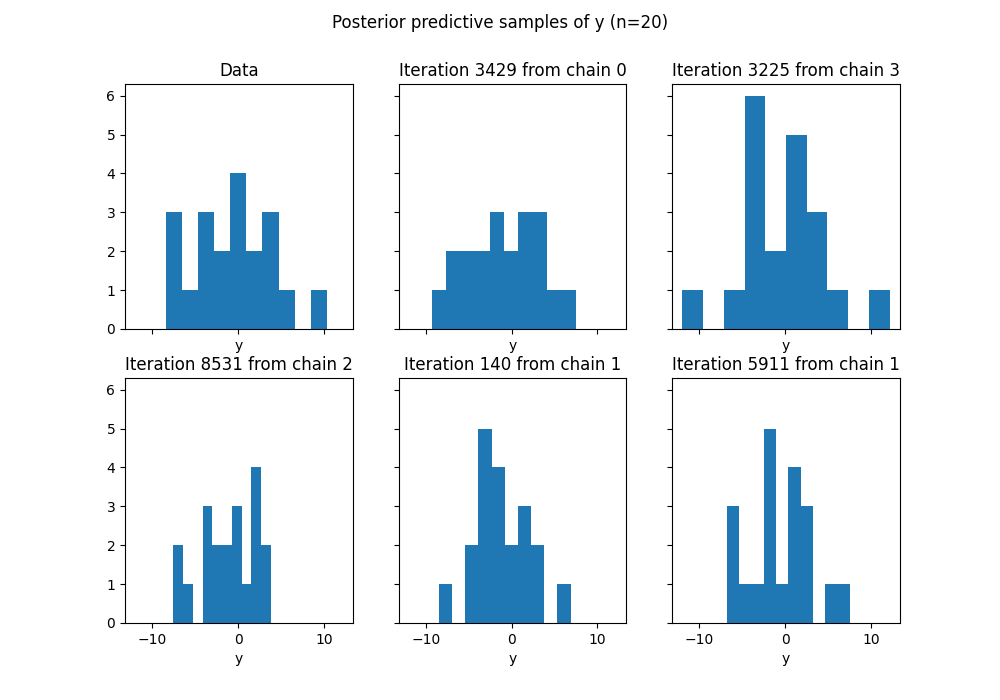
\includegraphics[height=.5\textwidth]{../outputs/artificial_scenarios_n=20/scenario_1/posterior_predictive_check.png}
        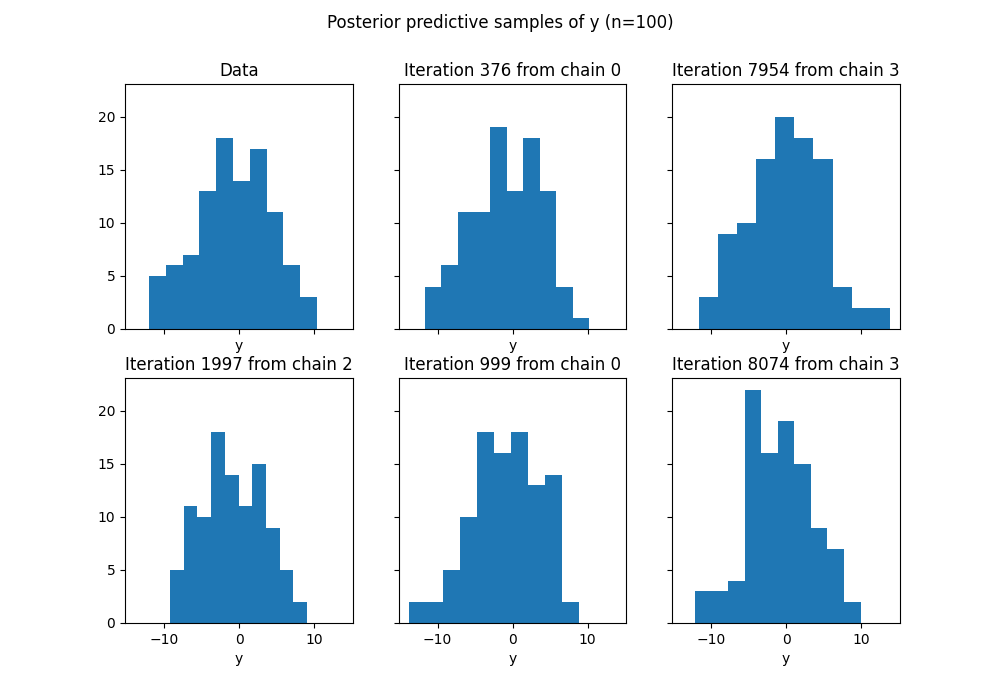
\includegraphics[height=.5\textwidth]{../outputs/artificial_scenarios_n=100/scenario_1/posterior_predictive_check.png}
    \end{center}
    \caption[Posterior predictive checks for Scenario 1.]{Posterior predictive checks for Scenario 1. The parameters corresponding to these $ 5$ (for each $ n $) simulated values from $ \by $ were randomly and uniformly chosen across all samples from the posterior.}
    \label{fig: posterior predictive check scenario 1}
\end{figure}

To assess shrinkage, we computed $ 95\% $ credibility intervals using the $ 2.5\% $ and $ 97.5\% $ quantiles of the $ 50 000 $ posterior samples.
We interpret that a parameter should be set to $ 0 $ when the corresponding $ 95\% $ credibility interval contains $ 0 $.
These are shown in Figure \ref{fig: credibility intervals scenario 1}.
For comparison, we also plotted the true $ \betabold_{ i } $ values, as well as the estimate produced by the classical LASSO when $ \lambda $ is chosen through cross validation.

We can see that, for the smaller sample size, the Bayesian LASSO correctly produced credibility intervals which are centered around $ 0 $ for the $ \betabold_{ i } $'s which were actually zero.
However, it had difficulty producing credibility intervals which clearly put the non-zero parameters away from zero, getting $ \betabold_{ 5 } $ completely wrong, for example.
On a positive note for Bayesians, the classical LASSO was guilty of the same mistakes, since its estimates always fell within the $ (25\%, 75\%) $ credibility interval of the Bayesian LASSO.
For the larger sample size, however, the Bayesian LASSO showed a significant improvement.
It managed to correctly separate the null parameters from the non-null ones, while the classical LASSO failed to set any parameter to $ 0 $.
\begin{figure}[htb]
    \begin{center}
        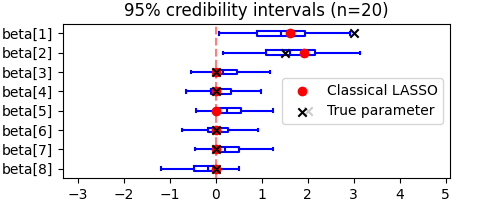
\includegraphics[width=.6\textwidth]{../outputs/artificial_scenarios_n=20/scenario_1/credibility_intervals.png}
        \vspace{1cm}
        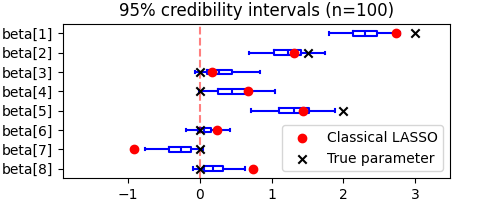
\includegraphics[width=.6\textwidth]{../outputs/artificial_scenarios_n=100/scenario_1/credibility_intervals.png}
    \end{center}
    \caption[95\% credibility intervals for Scenario 1.]{95\% credibility intervals for Scenario 1. The red dots are the classical LASSO's predictions when fit using cross validation, and the black crosses are the true parameter values. The vertical red line corresponds to $ x = 0 $.}
    \label{fig: credibility intervals scenario 1}
\end{figure}


\subsection*{Scenario 2}

For this scenario, the parameters were
\begin{align*}
    \betabold &= (0.85, 0.85, 0.85, 0.85, 0.85, 0.85, 0.85, 0.85) \\
    \sigma &= 3
.\end{align*}
The distribution of $ \bX $ was the same as in Scenario 1.
Effective sample sizes and $ \hat{ R } $ statistics are in Table \ref{tab: Eff and Rhat scenario 2}, while trace plots, posterior predictive checks and 95\% credibility intervals are in Figures \ref{fig: traceplots scenario 2}, \ref{fig: posterior predictive check scenario 2} and \ref{fig: credibility intervals scenario 2}, respectively.
\begin{table}[htb]
    \centering
    \begin{tabular}{lrr}
& $ n = 20 $ & \\
\toprule
 & N\_Eff & R\_hat \\
\midrule
lp\_\_ & 13250.000000 & 1.000000 \\
mu & 46830.000000 & 1.000000 \\
beta[1] & 29538.000000 & 1.000000 \\
beta[2] & 30893.000000 & 1.000000 \\
beta[3] & 32954.000000 & 1.000000 \\
beta[4] & 30811.000000 & 1.000000 \\
beta[5] & 32159.000000 & 1.000000 \\
beta[6] & 33505.000000 & 1.000000 \\
beta[7] & 28825.000000 & 1.000000 \\
beta[8] & 29206.000000 & 1.000000 \\
sigma & 34513.738000 & 1.000000 \\
lambda & 32343.862000 & 1.000000 \\
\bottomrule
\end{tabular}

    \quad
    \begin{tabular}{lrr}
& $ n = 100 $ & \\
\toprule
 & N\_Eff & R\_hat \\
\midrule
lp\_\_ & 22100.000000 & 1.000000 \\
mu & 53480.000000 & 0.999900 \\
beta[1] & 42594.000000 & 1.000000 \\
beta[2] & 38128.000000 & 1.000000 \\
beta[3] & 38743.000000 & 1.000000 \\
beta[4] & 33994.000000 & 1.000000 \\
beta[5] & 44015.000000 & 1.000000 \\
beta[6] & 35119.000000 & 1.000000 \\
beta[7] & 35445.000000 & 1.000000 \\
beta[8] & 39788.000000 & 1.000000 \\
sigma & 46622.085200 & 1.000100 \\
lambda & 52132.501200 & 0.999900 \\
\bottomrule
\end{tabular}

    \caption{Effective sample sizes and $ \hat{ R } $ statistics for Scenario 2, reported with four significant digits.}
    \label{tab: Eff and Rhat scenario 2}
\end{table}
\begin{figure}[htb]
    \begin{center}
        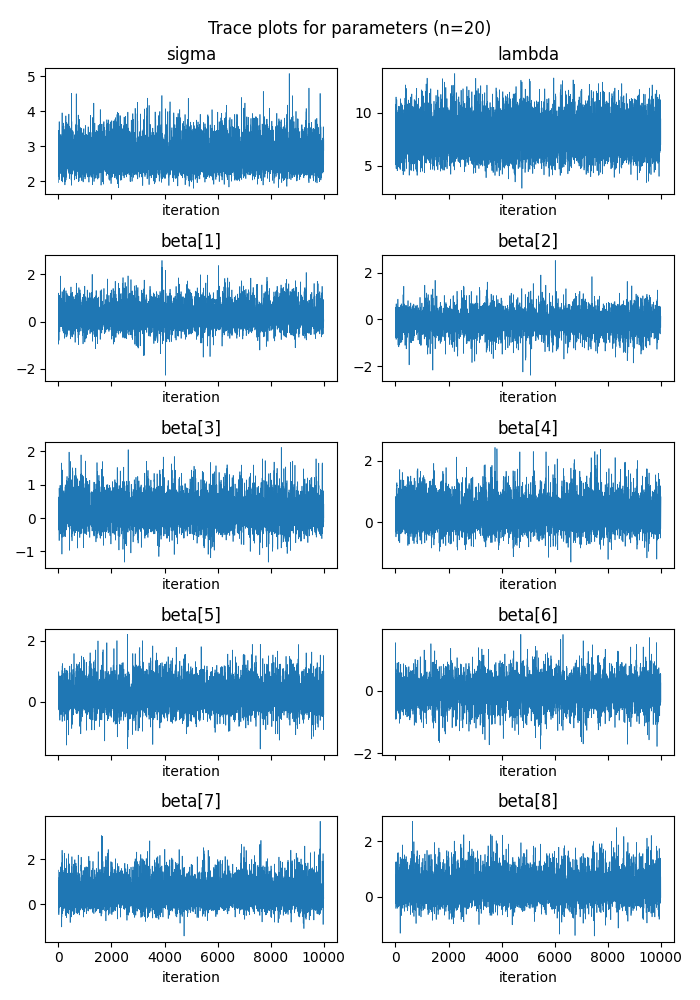
\includegraphics[height=.4\textheight]{../outputs/artificial_scenarios_n=20/scenario_2/traceplots.png}
        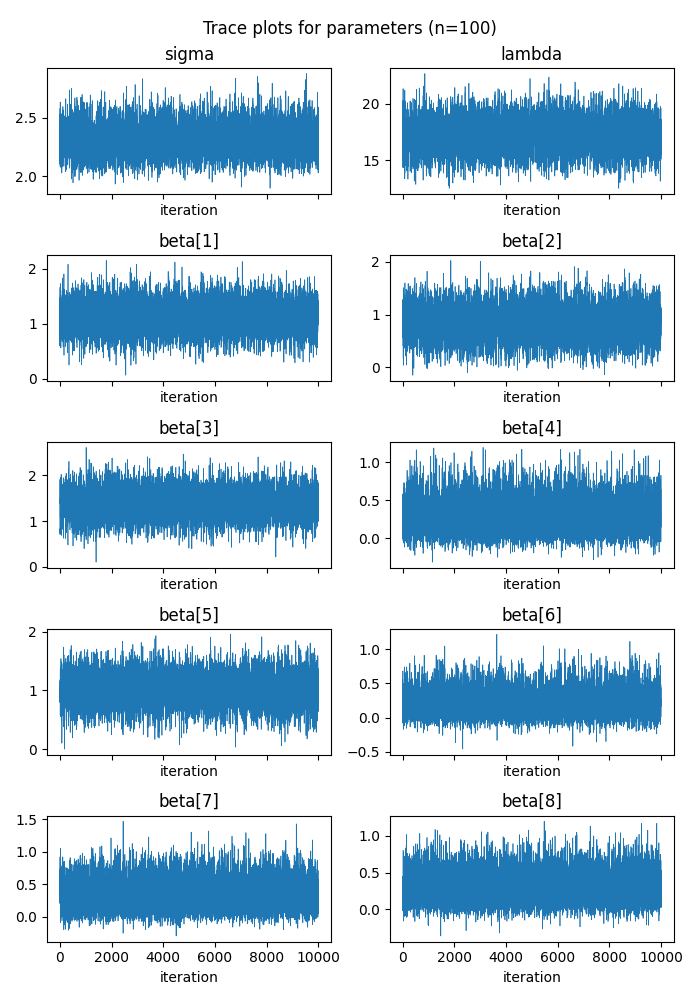
\includegraphics[height=.4\textheight]{../outputs/artificial_scenarios_n=100/scenario_2/traceplots.png}
    \end{center}
    \caption[Trace plots for the parameters in Scenario 2.]{Trace plots for the parameters in Scenario 2. Each plot is from one of the 5 chains, chosen randomly and uniformly.}
    \label{fig: traceplots scenario 2}
\end{figure}
\begin{figure}[htb]
    \begin{center}
        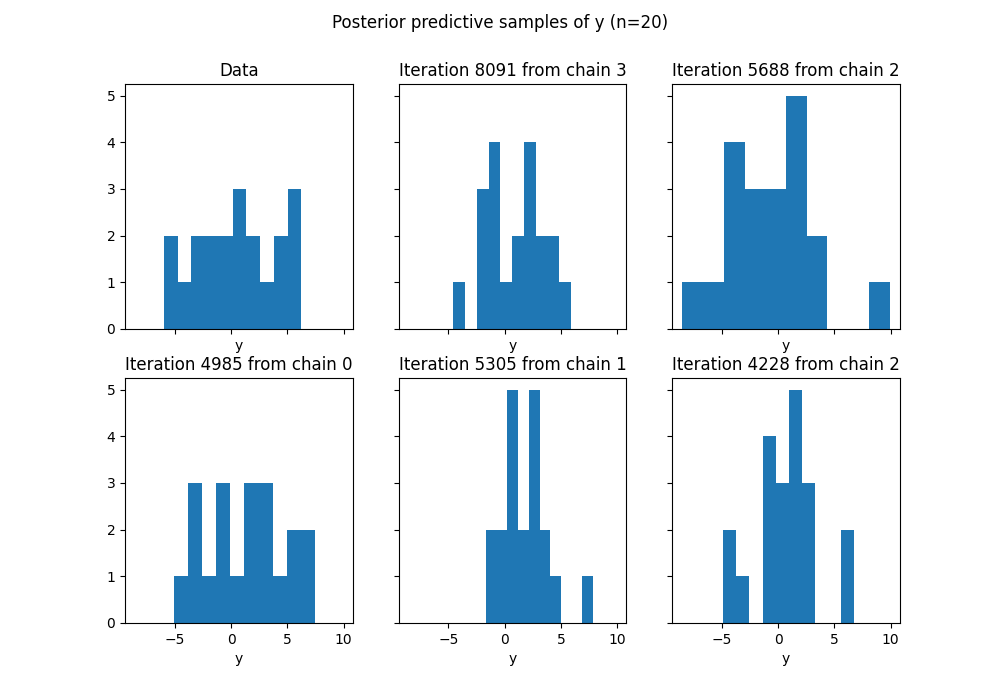
\includegraphics[height=.5\textwidth]{../outputs/artificial_scenarios_n=20/scenario_2/posterior_predictive_check.png}
        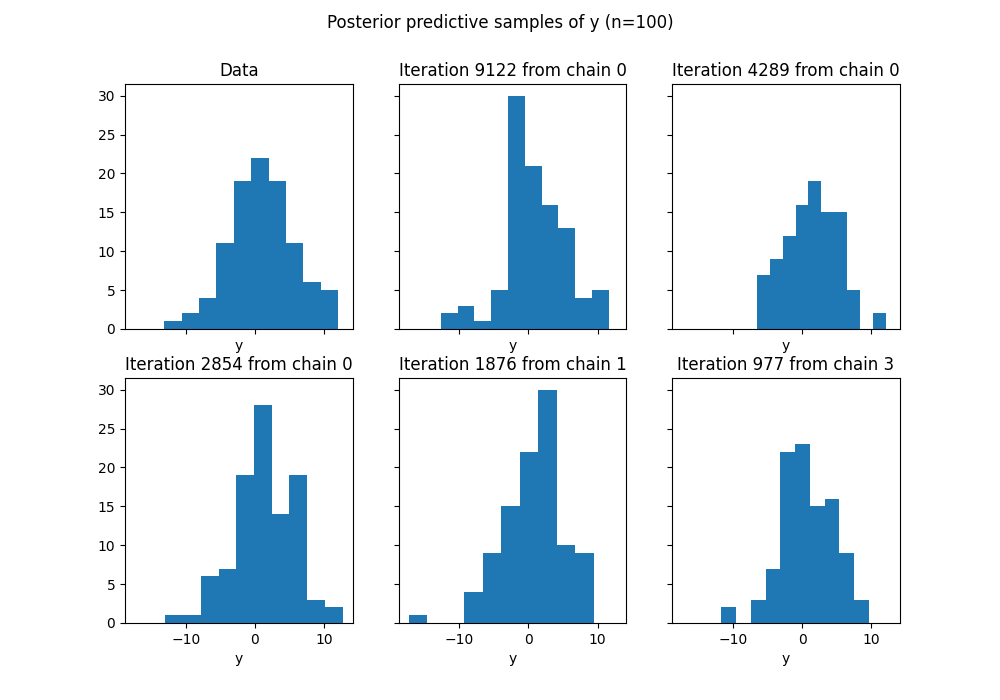
\includegraphics[height=.5\textwidth]{../outputs/artificial_scenarios_n=100/scenario_2/posterior_predictive_check.png}
    \end{center}
    \caption[Posterior predictive checks for Scenario 2.]{Posterior predictive checks for Scenario 2. The parameters corresponding to these $ 5$ (for each $ n $) simulated values from $ \by $ were randomly and uniformly chosen across all samples from the posterior.}
    \label{fig: posterior predictive check scenario 2}
\end{figure}
\begin{figure}[htb]
    \begin{center}
        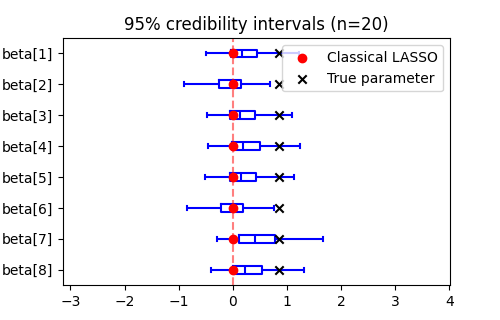
\includegraphics[width=.6\textwidth]{../outputs/artificial_scenarios_n=20/scenario_2/credibility_intervals.png}
        \vspace{1cm}
        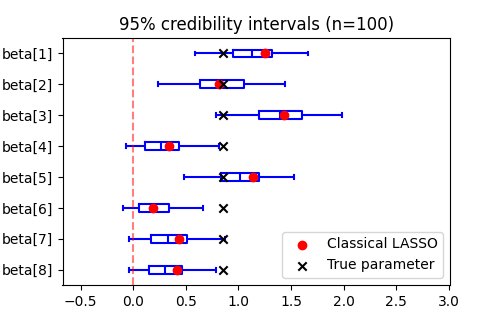
\includegraphics[width=.6\textwidth]{../outputs/artificial_scenarios_n=100/scenario_2/credibility_intervals.png}
    \end{center}
    \caption[95\% credibility intervals for Scenario 2.]{95\% credibility intervals for Scenario 2. The red dots are the classical LASSO's predictions when fit using cross validation, and the black crosses are the true parameter values. The vertical red line corresponds to $ x = 0 $.}
    \label{fig: credibility intervals scenario 2}
\end{figure}
Once again, effective sample sizes and $ \hat{ R } $ statistics are very healthy, as well as the trace plots.
The posterior predictive distribution for $ \by $ were again misaligned with the data for $ n = 20 $, but were much more faithful for $ n = 100 $.
This scenario differs from Scenario 1 in that \emph{no true coefficients were $ 0 $.}
This creates an awkward situation, in which, for $ n = 20 $, both the classical LASSO and the Bayesian LASSO shrunk all coefficients to $ 0 $, although it should be noted that all but two Bayesian LASSO credibility intervals correctly included the true $ \betabold_{ i } $ value.
When $ n = 100 $, however, the situation changes.
Four Bayesian LASSO credibility intervals correctly did not shrink the parameter to zero and included the true parameter value.
The other four wrongly included $ 0 $, but just barely.
Once again, for both sample sizes the classical LASSO estimates tended to fall within the $ (25\%, 75\%) $ credibility interval of the Bayesian LASSO.

\subsection*{Scenario 3}
For this scenario, the parameters were
\begin{align*}
    \betabold &= (5, 0, 0, 0, 0, 0, 0, 0) \\
    \sigma &= 2
.\end{align*}
The distribution of $ \bX $ was the same as in Scenarios 1 and 2.
Effective sample sizes and $ \hat{ R } $ statistics are in Table \ref{tab: Eff and Rhat scenario 3}, while trace plots, posterior predictive checks and 95\% credibility intervals are in Figures \ref{fig: traceplots scenario 3}, \ref{fig: posterior predictive check scenario 3} and \ref{fig: credibility intervals scenario 3}, respectively.
The comments about effective sample size, $ \hat{ R } $ statistics, trace plots and posterior predictive checks made previously also apply here.
\begin{table}[htb]
    \centering
    \begin{tabular}{lrr}
\toprule
 & N_Eff & R_hat \\
\midrule
lp__ & 15020.000000 & 1.001000 \\
mu & 45560.000000 & 1.000000 \\
beta[1] & 29434.000000 & 1.000000 \\
beta[2] & 33079.000000 & 1.000000 \\
beta[3] & 39256.000000 & 1.000000 \\
beta[4] & 40002.000000 & 1.000000 \\
beta[5] & 40608.000000 & 1.000000 \\
beta[6] & 35598.000000 & 1.000000 \\
beta[7] & 41152.000000 & 1.000000 \\
beta[8] & 34751.000000 & 1.000000 \\
sigma & 28577.832000 & 1.000000 \\
lambda & 32480.464000 & 1.000000 \\
\bottomrule
\end{tabular}

    \quad
    \begin{tabular}{lrr}
& $ n = 100 $ & \\
\toprule
 & N\_Eff & R\_hat \\
\midrule
lp\_\_ & 16390.000000 & 1.000000 \\
mu & 49930.000000 & 0.999900 \\
beta[1] & 45798.000000 & 1.000000 \\
beta[2] & 39123.000000 & 1.000000 \\
beta[3] & 44796.000000 & 1.000000 \\
beta[4] & 40713.000000 & 1.000000 \\
beta[5] & 46209.000000 & 1.000000 \\
beta[6] & 41420.000000 & 1.000000 \\
beta[7] & 43684.000000 & 1.000000 \\
beta[8] & 42667.000000 & 0.999900 \\
sigma & 46355.200300 & 1.000100 \\
lambda & 46537.422700 & 1.000000 \\
\bottomrule
\end{tabular}

    \caption{Effective sample sizes and $ \hat{ R } $ statistics for Scenario 3, reported with four significant digits.}
    \label{tab: Eff and Rhat scenario 3}
\end{table}
\begin{figure}[htb]
    \begin{center}
        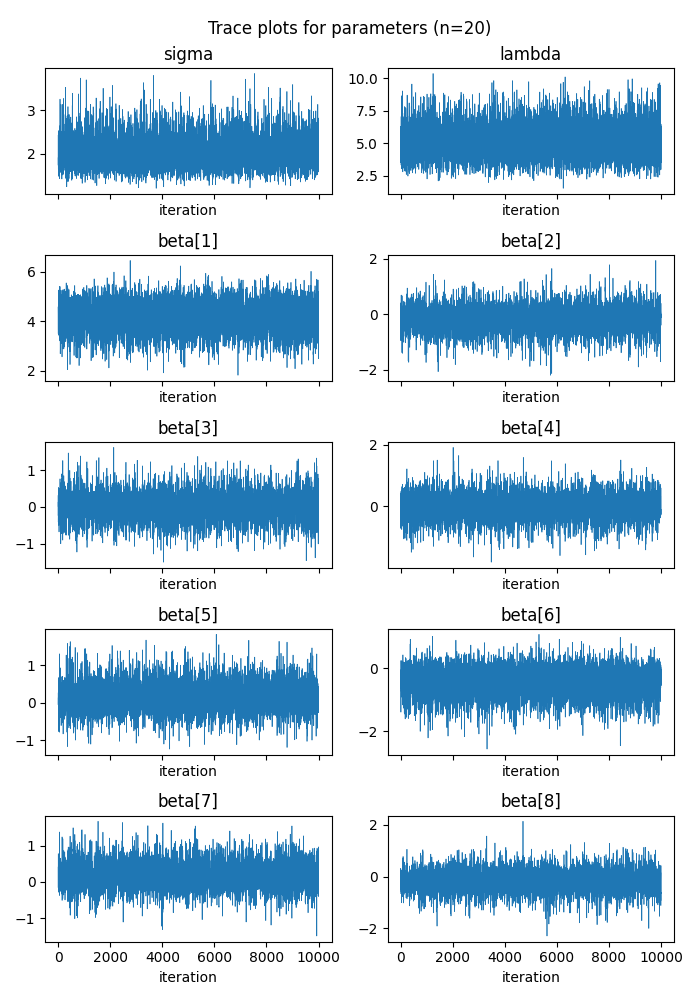
\includegraphics[height=.4\textheight]{../outputs/artificial_scenarios_n=20/scenario_3/traceplots.png}
        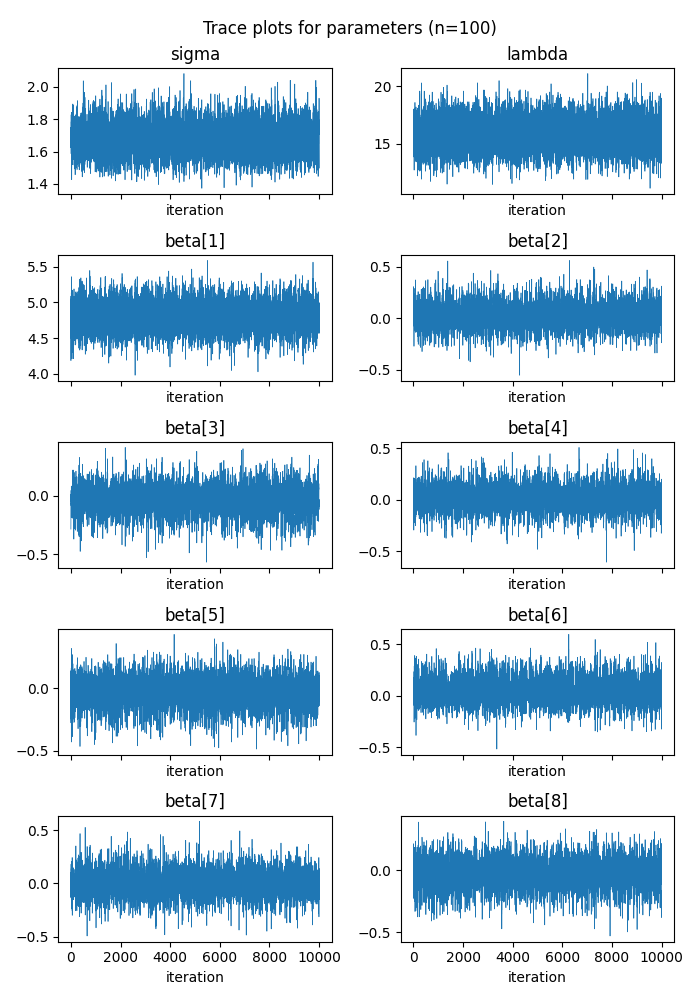
\includegraphics[height=.4\textheight]{../outputs/artificial_scenarios_n=100/scenario_3/traceplots.png}
    \end{center}
    \caption[Trace plots for the parameters in Scenario 3.]{Trace plots for the parameters in Scenario 3. Each plot is from one of the 5 chains, chosen randomly and uniformly.}
    \label{fig: traceplots scenario 3}
\end{figure}
\begin{figure}[htb]
    \begin{center}
        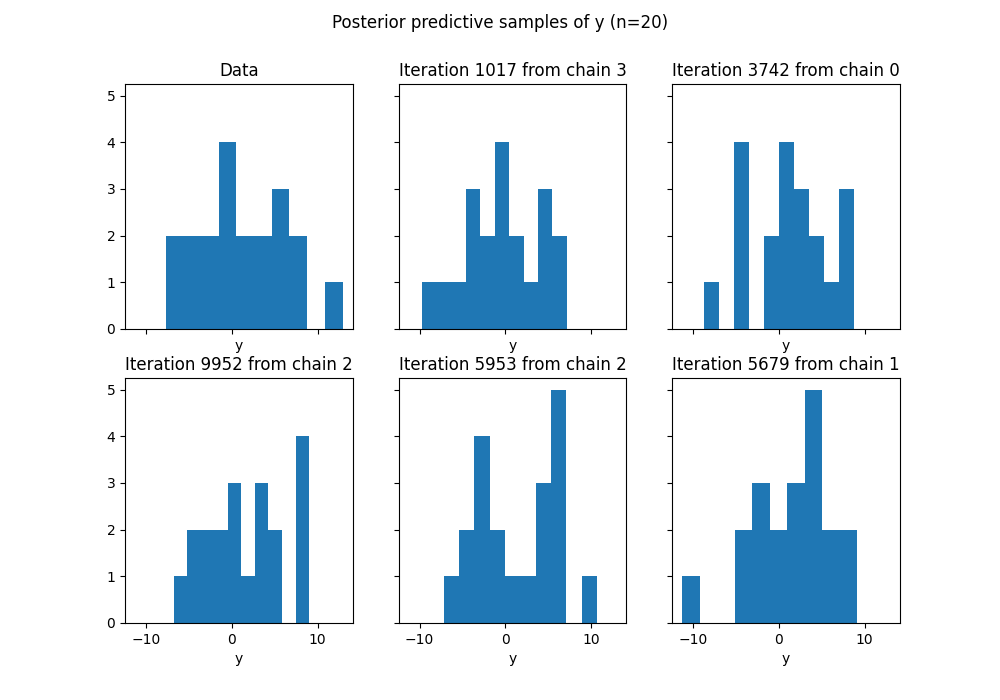
\includegraphics[height=.5\textwidth]{../outputs/artificial_scenarios_n=20/scenario_3/posterior_predictive_check.png}
        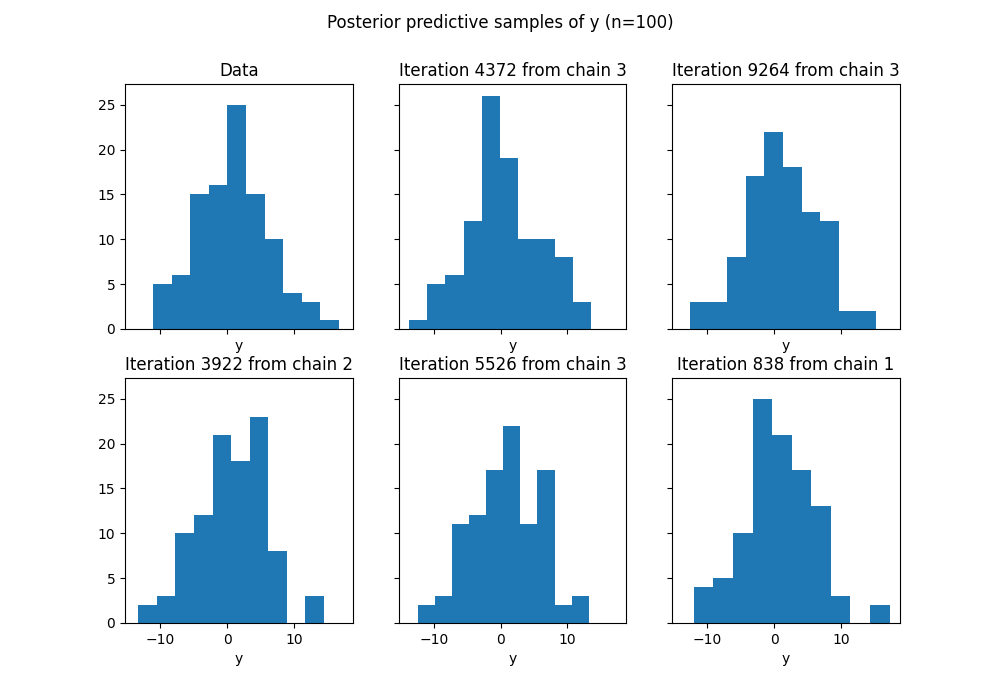
\includegraphics[height=.5\textwidth]{../outputs/artificial_scenarios_n=100/scenario_3/posterior_predictive_check.png}
    \end{center}
    \caption[Posterior predictive checks for Scenario 3.]{Posterior predictive checks for Scenario 3. The parameters corresponding to these $ 5$ (for each $ n $) simulated values from $ \by $ were randomly and uniformly chosen across all samples from the posterior.}
    \label{fig: posterior predictive check scenario 3}
\end{figure}
\begin{figure}[htb]
    \begin{center}
        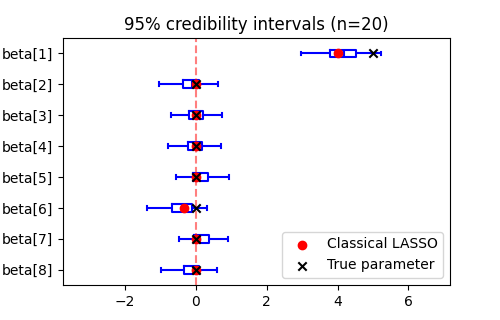
\includegraphics[width=.6\textwidth]{../outputs/artificial_scenarios_n=20/scenario_3/credibility_intervals.png}
        \vspace{1cm}
        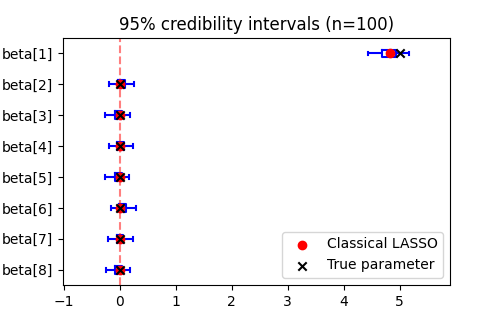
\includegraphics[width=.6\textwidth]{../outputs/artificial_scenarios_n=100/scenario_3/credibility_intervals.png}
    \end{center}
    \caption[95\% credibility intervals for Scenario 3.]{95\% credibility intervals for Scenario 3. The red dots are the classical LASSO's predictions when fit using cross validation, and the black crosses are the true parameter values. The vertical red line corresponds to $ x = 0 $.}
    \label{fig: credibility intervals scenario 3}
\end{figure}

This scenario is much more friendly for sparse regression methods, since the variance of $ \by $ is smaller and almost all coefficients are exactly $ 0 $, except for $ \betabold_{ 1 } $, which is considerably large, given the scale of $ \bX $.
This is apparent in the credibility intervals, which managed to always include the true parameter value, as well as shrink only the parameters which were actually $ 0 $.
The increase in sample size only decreased the size of the intervals.
The classical LASSO also had a good performance, staying very close to the median of the Bayesian LASSO.

\subsection*{Scenario 4}
For this scenario, the parameters were
\begin{align*}
    \betabold &= (0, 0, \dots, 0, 2, 2, \dots, 2, 0, 0, \dots, 0, 2, 2, \dots, 2) \\
    \sigma &= 15
,\end{align*}
where each block in $ \betabold $ has size 10, meaning the total number of covariates is $ p = 40 $.
The correlation between different predictors was set to $ 0.5 $.
Since this model is much larger than the other three, the sample sizes we analyzed were $ n = 100 $ and $ n = 500 $.
Effective sample sizes and $ \hat{ R } $ statistics are in Table \ref{tab: Eff and Rhat scenario 4}, while posterior predictive checks and 95\% credibility intervals are in Figures \ref{fig: posterior predictive check scenario 4} and \ref{fig: credibility intervals scenario 4}, respectively.
Given the number of covariates, we did not analyze trace plots.
The comments about effective sample size, $ \hat{ R } $ statistics and posterior predictive checks made previously also apply here.
\begin{table}[htb]
    \centering
    \begin{tabular}{lrr}
\toprule
 & N_Eff & R_hat \\
\midrule
lp__ & 14530.000000 & 1.000000 \\
mu & 49030.000000 & 1.000000 \\
beta[1] & 29664.000000 & 1.000000 \\
beta[2] & 31146.000000 & 1.000000 \\
beta[3] & 32062.000000 & 1.000000 \\
beta[4] & 39290.000000 & 1.000000 \\
beta[5] & 34542.000000 & 1.000000 \\
beta[6] & 34233.000000 & 1.000000 \\
beta[7] & 36328.000000 & 1.000000 \\
beta[8] & 32915.000000 & 1.000000 \\
beta[9] & 30429.000000 & 1.000000 \\
beta[10] & 29737.000000 & 1.000000 \\
beta[11] & 28833.000000 & 1.000000 \\
beta[12] & 29526.000000 & 1.000000 \\
beta[13] & 29834.000000 & 1.000000 \\
beta[14] & 33105.000000 & 1.000000 \\
beta[15] & 32283.000000 & 1.000000 \\
beta[16] & 37561.000000 & 1.000000 \\
beta[17] & 32573.000000 & 1.000000 \\
beta[18] & 33255.000000 & 1.000000 \\
beta[19] & 28352.000000 & 1.000000 \\
beta[20] & 29985.000000 & 1.000000 \\
beta[21] & 31635.000000 & 1.000000 \\
beta[22] & 31775.000000 & 1.000000 \\
beta[23] & 34241.000000 & 1.000000 \\
beta[24] & 27634.000000 & 1.000000 \\
beta[25] & 35355.000000 & 1.000000 \\
beta[26] & 28754.000000 & 1.000000 \\
beta[27] & 33787.000000 & 1.000000 \\
beta[28] & 37865.000000 & 1.000000 \\
beta[29] & 38216.000000 & 1.000000 \\
beta[30] & 38568.000000 & 1.000000 \\
beta[31] & 30802.000000 & 1.000000 \\
beta[32] & 27095.000000 & 1.000000 \\
beta[33] & 26375.000000 & 1.000000 \\
beta[34] & 27281.000000 & 1.000000 \\
beta[35] & 29202.000000 & 1.000000 \\
beta[36] & 31880.000000 & 1.000000 \\
beta[37] & 32594.000000 & 1.000000 \\
beta[38] & 31836.000000 & 1.000000 \\
beta[39] & 31113.000000 & 1.000000 \\
beta[40] & 29106.000000 & 1.000000 \\
sigma & 35637.644000 & 1.000000 \\
lambda & 34152.046000 & 1.000000 \\
\bottomrule
\end{tabular}

    \quad
    \begin{tabular}{lrr}
& $ n = 500 $ & \\
\toprule
 & N\_Eff & R\_hat \\
\midrule
lp\_\_ & 17720.000000 & 1.000000 \\
mu & 39490.000000 & 1.000000 \\
beta[1] & 35021.000000 & 1.000000 \\
beta[2] & 34017.000000 & 1.000000 \\
beta[3] & 34293.000000 & 1.000000 \\
beta[4] & 32462.000000 & 1.000000 \\
beta[5] & 30194.000000 & 1.000000 \\
beta[6] & 29062.000000 & 1.000000 \\
beta[7] & 27408.000000 & 1.000000 \\
beta[8] & 27918.000000 & 1.000000 \\
beta[9] & 26745.000000 & 1.000000 \\
beta[10] & 24627.000000 & 1.000000 \\
beta[11] & 37007.000000 & 1.000000 \\
beta[12] & 37694.000000 & 1.000000 \\
beta[13] & 40944.000000 & 1.000000 \\
beta[14] & 33475.000000 & 1.000000 \\
beta[15] & 32878.000000 & 1.000000 \\
beta[16] & 37431.000000 & 1.000000 \\
beta[17] & 38631.000000 & 1.000000 \\
beta[18] & 36876.000000 & 1.000000 \\
beta[19] & 39417.000000 & 1.000000 \\
beta[20] & 36417.000000 & 1.000000 \\
beta[21] & 26103.000000 & 1.000000 \\
beta[22] & 37153.000000 & 1.000000 \\
beta[23] & 28222.000000 & 1.000000 \\
beta[24] & 27295.000000 & 1.000000 \\
beta[25] & 28212.000000 & 1.000000 \\
beta[26] & 33869.000000 & 1.000000 \\
beta[27] & 31385.000000 & 1.000000 \\
beta[28] & 24276.000000 & 1.000000 \\
beta[29] & 36815.000000 & 1.000000 \\
beta[30] & 26786.000000 & 1.000000 \\
beta[31] & 36241.000000 & 1.000000 \\
beta[32] & 36215.000000 & 1.000000 \\
beta[33] & 32350.000000 & 1.000000 \\
beta[34] & 28491.000000 & 1.000000 \\
beta[35] & 38596.000000 & 1.000000 \\
beta[36] & 26368.000000 & 1.000000 \\
beta[37] & 28086.000000 & 1.000000 \\
beta[38] & 37653.000000 & 1.000000 \\
beta[39] & 38766.000000 & 1.000000 \\
beta[40] & 37611.000000 & 1.000000 \\
sigma & 39951.620600 & 1.000100 \\
lambda & 42298.545900 & 1.000100 \\
\bottomrule
\end{tabular}

    \caption{Effective sample sizes and $ \hat{ R } $ statistics for Scenario 4, reported with four significant digits.}
    \label{tab: Eff and Rhat scenario 4}
\end{table}
\begin{figure}[htb]
    \begin{center}
        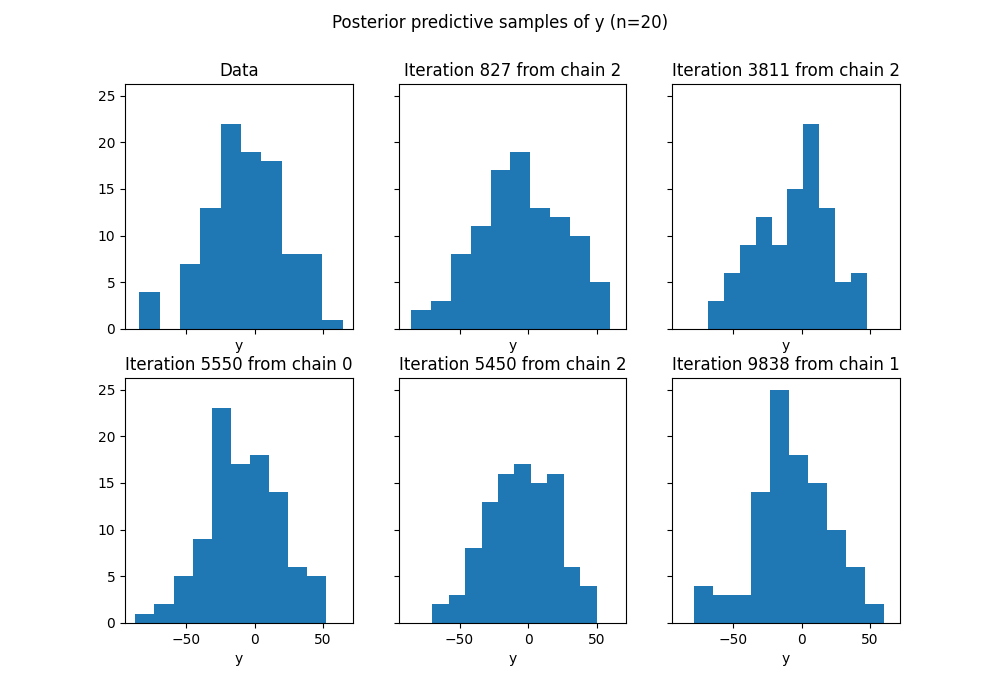
\includegraphics[height=.5\textwidth]{../outputs/artificial_scenarios_n=20/scenario_4/posterior_predictive_check.png}
        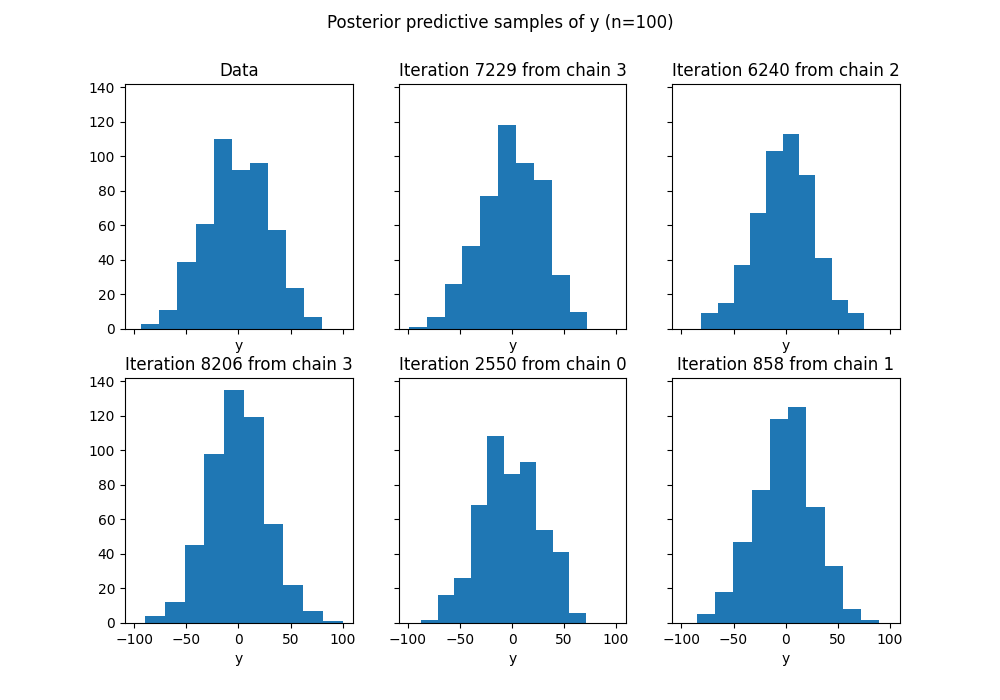
\includegraphics[height=.5\textwidth]{../outputs/artificial_scenarios_n=100/scenario_4/posterior_predictive_check.png}
    \end{center}
    \caption[Posterior predictive checks for Scenario 4.]{Posterior predictive checks for Scenario 4. The parameters corresponding to these $ 5$ (for each $ n $) simulated values from $ \by $ were randomly and uniformly chosen across all samples from the posterior.}
    \label{fig: posterior predictive check scenario 4}
\end{figure}
\begin{figure}[htb]
    \begin{center}
        \vspace{-4cm}
        \begin{minipage}{.47\textwidth}
            \centering
            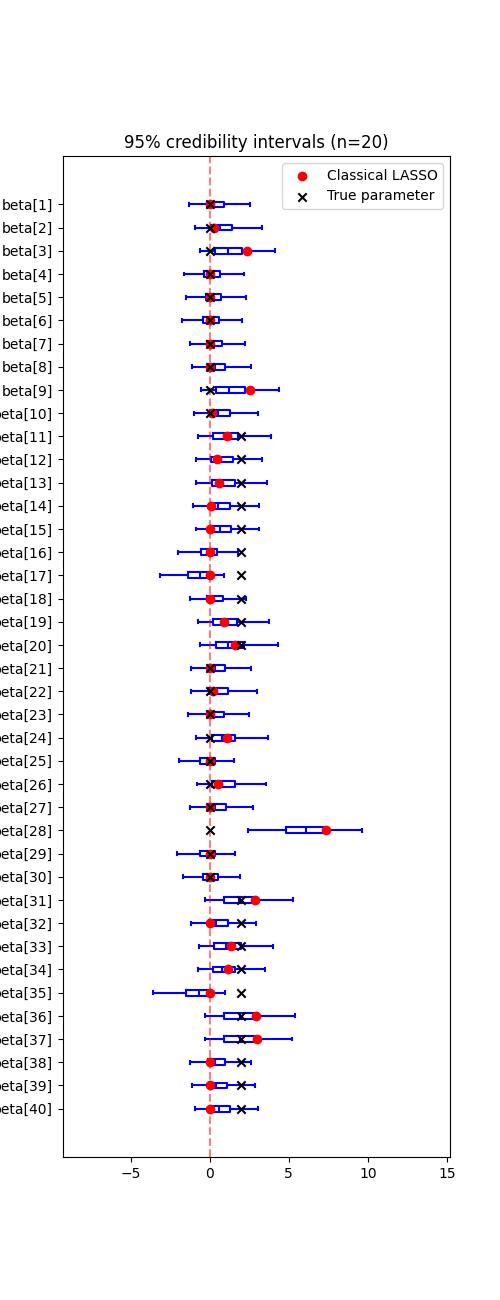
\includegraphics[width=\textwidth]{../outputs/artificial_scenarios_n=20/scenario_4/credibility_intervals.png}
        \end{minipage}%
        \begin{minipage}{.47\textwidth}
            \centering
            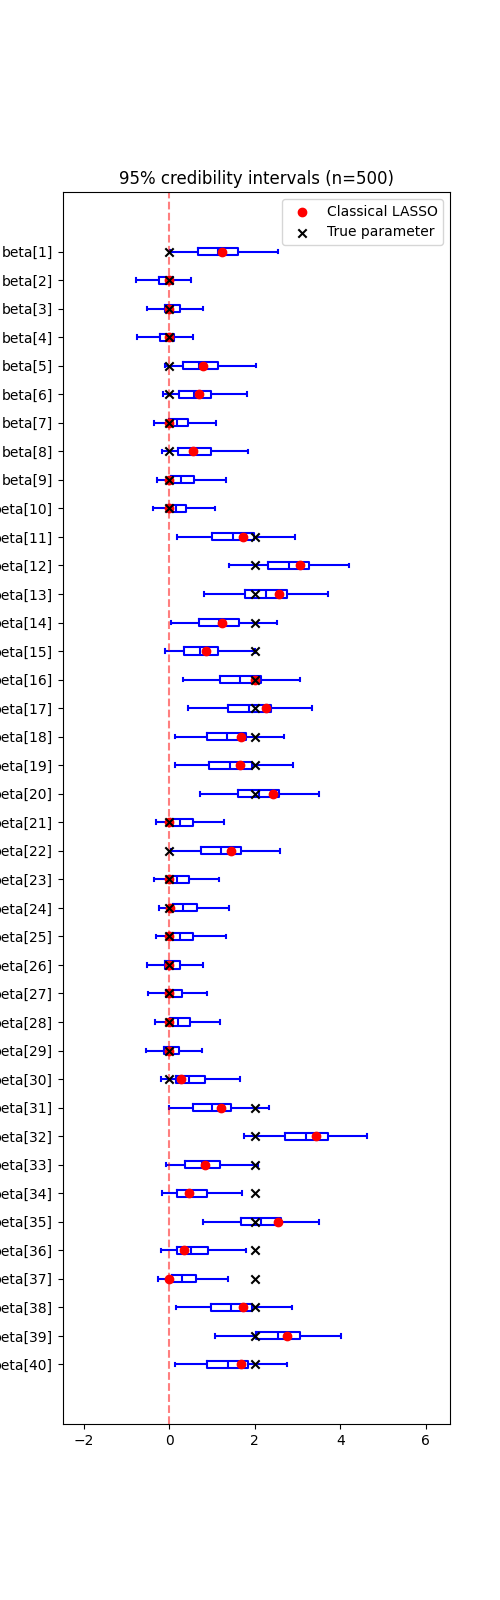
\includegraphics[width=\textwidth]{../outputs/artificial_scenarios_n=100/scenario_4/credibility_intervals.png}
        \end{minipage}
    \end{center}
    \caption[95\% credibility intervals for Scenario 4.]{95\% credibility intervals for Scenario 4. The red dots are the classical LASSO's predictions when fit using cross validation, and the black crosses are the true parameter values. The vertical red line corresponds to $ x = 0 $.}
    \label{fig: credibility intervals scenario 4}
\end{figure}
While all diagnostics employed indicate our sampling scheme is performing as intended, the Bayesian LASSO faced great difficulty in this scenario, collapsing all but two covariates to $ 0 $ in the $ n = 100 $ regime.
In this sample size, the classical LASSO showed a better performance in terms of shrinkage, managing to correctly not collapse $ 14 $ non-zero parameters, in spite of failing to collapse $ 2 $ actually null ones.
When $ n $ was increased to $ 500 $, the credibility intervals for the parameters equal to $ 2 $ generally shifted towards the positive side, but this was still not enough to correctly decide which parameters are actually $ 0 $.
These results show that the Bayesian LASSO may face difficulties when $ p $ is large and the proportion of non-null parameters is high.



% For each scenario:
% \begin{itemize}
%     \item Show table with Stan summary;
%     \item Show trace plots of chains for all parameters;
%     \item Show prior and posterior predictive distributions;
%     \item Show graph with 95\% confidence intervals for all parameters;
% \end{itemize}


\section{Choosing $\lambda$}
\label{sec: diabetes data experiment}

In\footnote{Corresponds to item f).} \cite{parkcasella2008bayesianlasso}, two approaches are presented to ``choose'' the LASSO parameter $ \lambda $.
The first one is based on an EM algorithm to choose the $ \lambda $ value which maximizes the marginal likelihood of the data.
The second one is arguably more suitable for a Bayesian analysis\footnote{And is considerably easier to implement using \texttt{Stan} \emoji{grinning-face-with-sweat}.} and consists of simply incorporating $ \lambda $ as an additional pararameter.
As was seen in the previous section, we chose to use the second option for our experiments.
To maintain conjugacy, one should specify a Gamma prior on $ \lambda^2 $ \cite{parkcasella2008bayesianlasso}.
However, the choice of hyperparameters for this prior in \cite{parkcasella2008bayesianlasso} was based on a desired relationship between the prior mean and the MLE.
This makes little sense in the Bayesian context, as the prior should not be chosen based on information gained from the data values.

To analyze what effects the choice of the $ \lambda $ hyperprior hyperparameters has on the final estimate, we applied the Bayesian Lasso to the \texttt{diabetes} dataset of \cite{effron-2004-diabetes} using three combinations of hyperparameters.
The hyperprior was $ \lambda^2 \sim \distgamma (\delta, r) $.
The computational tools used to fit the models were the same ones described in Section \ref{sec: artificial data experiments}.

\begin{itemize}
    \item $ \delta = 1, r = 1.78: $
    These are the hyperparameters suggested in \cite{parkcasella2008bayesianlasso}.
    Summary statistics are presented in Table \ref{tab: diabetes summary scenario 1} and credibility intervals can be visualized in Figure \ref{fig: diabetes credibility scenario 1}.
    Interestingly enough, our $ 95\% $, equal-tailed credibility interval for $ \lambda $ was $ ( 10.06, 11.498 ) $, completely different from the one reported in \cite{parkcasella2008bayesianlasso} of $ ( 0.139, 0.486  ) $.
    Since our $ \hat{ R } $ values are all close to $ 1 $ and the effective sample sizes surpass 25k for all variables, we have no reason to doubt our results.
    \begin{table}[htb]
        \centering
        \begin{tabular}{lrrrrr}
\toprule
 & 2.5\textbackslash \% & 50\textbackslash \% & 97.5\textbackslash \% & N\_Eff & R\_hat \\
\midrule
lp\_\_ & -2850.000000 & -2843.000000 & -2839.000000 & 20490.000000 & 1.000000 \\
mu & 148.300000 & 152.100000 & 155.600000 & 64750.000000 & 1.000000 \\
beta[1] & -3.628000 & -0.091650 & 3.040000 & 62712.000000 & 1.000000 \\
beta[2] & -13.730000 & -9.503000 & -5.623000 & 58193.000000 & 1.000000 \\
beta[3] & 20.230000 & 24.950000 & 29.180000 & 58450.000000 & 1.000000 \\
beta[4] & 9.721000 & 14.260000 & 18.440000 & 58566.000000 & 1.000000 \\
beta[5] & -15.180000 & -5.186000 & 1.582000 & 23732.000000 & 1.000000 \\
beta[6] & -8.897000 & -1.252000 & 4.845000 & 30117.000000 & 1.000000 \\
beta[7] & -15.730000 & -8.760000 & -1.482000 & 26419.000000 & 1.000000 \\
beta[8] & -3.072000 & 2.991000 & 11.270000 & 31179.000000 & 1.000000 \\
beta[9] & 17.840000 & 23.810000 & 29.430000 & 37253.000000 & 1.000000 \\
beta[10] & -1.067000 & 2.696000 & 6.847000 & 56814.000000 & 1.000000 \\
sigma & 36.946300 & 38.781400 & 40.606400 & 74059.453500 & 0.999900 \\
lambda & 10.059600 & 10.798400 & 11.498100 & 70911.294400 & 1.000000 \\
\bottomrule
\end{tabular}

        \caption{Summary statistics for the hyperparameters $ \delta = 1 $ and $ r = 1.78 $.}
        \label{tab: diabetes summary scenario 1}
    \end{table}
\begin{figure}
    \centering
    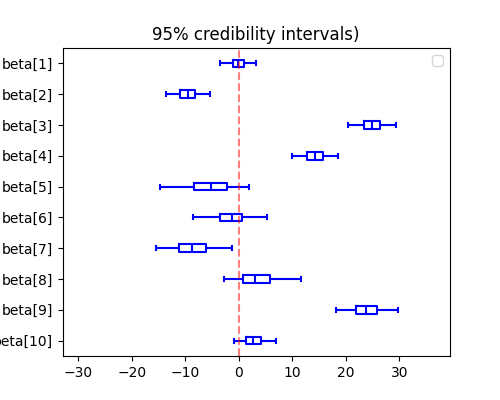
\includegraphics[width=.6\textwidth]{../outputs/diabetes_data/scenario_1/credibility_intervals.png}
    \caption{95\% credibility intervals for Diabetes data with $ \delta = 1 $ and $ r = 1.78 $.}
    \label{fig: diabetes credibility scenario 1}
\end{figure}

    \item $ \delta = 1.0, r = 0.1: $
    These are the hyperparameter values we used in Section \ref{sec: artificial data experiments}.
    Summary statistics are presented in Table \ref{tab: diabetes summary scenario 2} and credibility intervals can be visualized in Figure \ref{fig: diabetes credibility scenario 2}.
    The $ 95\% $ credibility interval we obtain for $ \lambda $ using these values is $ ( 39.54, 45.54 ) $.
    This is to be expected since the prior is way more diffuse and assigns more probability for larger values of $ \lambda $.
    \begin{table}[htb]
        \centering
        \begin{tabular}{lrrrrr}
\toprule
 & 2.5\textbackslash \% & 50\textbackslash \% & 97.5\textbackslash \% & N\_Eff & R\_hat \\
\midrule
lp\_\_ & -2282.000000 & -2275.000000 & -2271.000000 & 18320.000000 & 1.000000 \\
mu & 148.100000 & 152.100000 & 155.800000 & 48840.000000 & 1.000000 \\
beta[1] & -2.120000 & 0.044360 & 2.117000 & 38068.000000 & 1.000000 \\
beta[2] & -8.704000 & -4.295000 & -0.559700 & 34044.000000 & 1.000000 \\
beta[3] & 19.480000 & 24.270000 & 28.660000 & 35405.000000 & 1.000000 \\
beta[4] & 6.507000 & 11.250000 & 15.480000 & 33648.000000 & 1.000000 \\
beta[5] & -5.095000 & -0.849800 & 1.059000 & 21870.000000 & 1.000000 \\
beta[6] & -4.232000 & -0.699300 & 1.133000 & 27689.000000 & 1.000000 \\
beta[7] & -12.620000 & -7.433000 & -2.497000 & 25298.000000 & 1.000000 \\
beta[8] & -1.333000 & 0.866200 & 5.211000 & 21181.000000 & 1.000000 \\
beta[9] & 16.220000 & 21.450000 & 26.290000 & 33718.000000 & 1.000000 \\
beta[10] & -0.778000 & 1.429000 & 5.136000 & 31419.000000 & 1.000000 \\
sigma & 38.602000 & 40.575000 & 42.532000 & 41530.225000 & 1.000000 \\
lambda & 39.537000 & 42.611000 & 45.542000 & 44663.473000 & 1.000000 \\
\bottomrule
\end{tabular}

        \caption{Summary statistics for the hyperparameters $ \delta = 1 $ and $ r = 0.1 $.}
        \label{tab: diabetes summary scenario 2}
    \end{table}
\begin{figure}
    \centering
    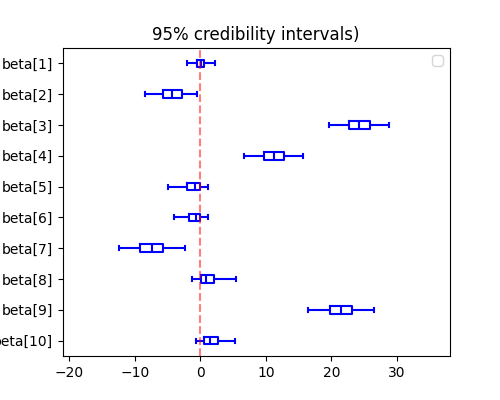
\includegraphics[width=.6\textwidth]{../outputs/diabetes_data/scenario_2/credibility_intervals.png}
    \caption{95\% credibility intervals for Diabetes data with $ \delta = 1 $ and $ r = 0.1 $.}
    \label{fig: diabetes credibility scenario 2}
\end{figure}

    \item $ \delta = 1.0, r = 10.0: $
    These hyperparameter values correspond to an informative prior which puts $ \lambda^2 $ close to zero, meaning the shrinking effect is smaller.
    Summary statistics are presented in Table \ref{tab: diabetes summary scenario 3} and credibility intervals can be visualized in Figure \ref{fig: diabetes credibility scenario 3}.
    The $ 95\% $ credibility interval we obtain for $ \lambda $ using these values is $ ( 4.31, 4.63 ) $.
    \begin{table}[htb]
        \centering
        \begin{tabular}{lrrrrr}
\toprule
 & 2.5\textbackslash \% & 50\textbackslash \% & 97.5\textbackslash \% & N\_Eff & R\_hat \\
\midrule
lp\_\_ & -3216.000000 & -3210.000000 & -3206.000000 & 21540.000000 & 1.000000 \\
mu & 148.400000 & 152.100000 & 155.600000 & 58280.000000 & 1.000000 \\
beta[1] & -4.074000 & -0.203500 & 3.227000 & 54814.000000 & 1.000000 \\
beta[2] & -14.770000 & -10.560000 & -6.703000 & 55482.000000 & 0.999900 \\
beta[3] & 20.400000 & 25.000000 & 29.200000 & 51029.000000 & 1.000000 \\
beta[4] & 10.390000 & 14.880000 & 19.010000 & 53606.000000 & 1.000000 \\
beta[5] & -27.930000 & -10.440000 & 1.294000 & 20926.000000 & 1.000000 \\
beta[6] & -9.521000 & 1.161000 & 14.490000 & 23264.000000 & 1.000000 \\
beta[7] & -15.700000 & -6.624000 & 1.620000 & 25770.000000 & 1.000000 \\
beta[8] & -3.622000 & 4.713000 & 13.680000 & 38928.000000 & 1.000000 \\
beta[9] & 18.560000 & 25.730000 & 33.190000 & 26433.000000 & 1.000000 \\
beta[10] & -1.140000 & 3.042000 & 7.202000 & 53886.000000 & 1.000000 \\
sigma & 36.592800 & 38.420700 & 40.227500 & 55799.672500 & 1.000000 \\
lambda & 4.311800 & 4.632000 & 4.928400 & 57694.368400 & 0.999900 \\
\bottomrule
\end{tabular}

        \caption{Summary statistics for the hyperparameters $ \delta = 1 $ and $ r = 10 $.}
        \label{tab: diabetes summary scenario 3}
    \end{table}
\begin{figure}
    \centering
    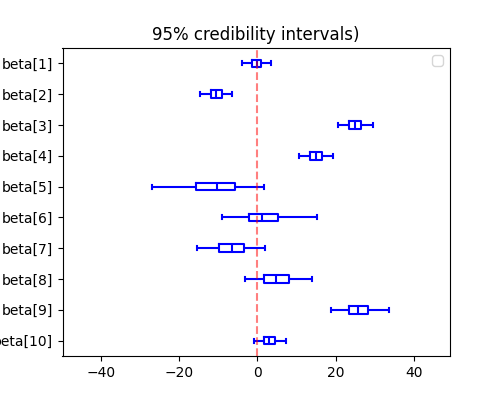
\includegraphics[width=.6\textwidth]{../outputs/diabetes_data/scenario_3/credibility_intervals.png}
    \caption{95\% credibility intervals for Diabetes data with $ \delta = 1 $ and $ r = 10 $.}
    \label{fig: diabetes credibility scenario 3}
\end{figure}
\end{itemize}
It is worth noting that the credibility intervals did not change considerably while varying the hyperparameter values.
In all three cases, only the parameters $ \betabold_{ 2 }, \betabold_{ 3 }, \betabold_{ 4 } $ and $ \betabold_{ 9 } $ were not collapsed to $ 0 $, while the median of the other parameters was similar across hyperparameter values.
This indicates that the model is robust to the choice of prior, which is a desirable feature.


\printbibliography

\end{document}